%**************************************************************
% CAPITOLO 3
%**************************************************************
\chapter{Il progetto di e-commerce VR}
\label{cap:ilprogettoe-commercevr}

\section{Analisi dei requisiti}

Questa sezione tratta dei casi d'uso e dei requisiti che il \textit{team} ha ricavato durante la discussione nella prima riunione di stage. Tale analisi ha subito un sostanzioso cambiamento durante la settimana 6, settimana dedicata alla prototipazione del possibile processo d'acquisto all'interno dell'ambiente virtuale. A causa della sua scarsa usabilità, abbiamo deciso di non utilizzare una tastiera virtuale all'interno dell'ambiente tridimensionale per dare la possibilità all'utente di immettere i propri dati e gli estremi di pagamento. Ciò ha portato il \textit{team} a prevedere una registrazione ad un normale sito di \textit{e-commerce} prima di effettuare l'autenticazione all'app, dove dar la possibilità all'utente di immettere i propri dati di pagamento. La sezione 3.2.2 spiega in maniera approfondita le sperimentazioni e le discussioni effettuate che hanno portato a questa importante decisione. 


\subsection{Caratteristiche degli utenti}

Obbligare l'utente ad immettere dati sensibili e strettamente personali, come gli estremi di pagamento, prima dell'effettivo utilizzo del servizio non è una buona prassi. L'utente, che si appresta per la prima volta ad utilizzare l'applicazione, potrebbe non conoscere l'azienda di produzione e potrebbe non fidarsi. Dunque sono stati delineati due principali tipologie d'utente:

\begin{itemize}
	\item \textbf{Utente registrato visitatore:} utente che ha effettuato la registrazione ma che ha deciso di non immettere i propri dati della carta di credito. Ad esso è permesso visualizzare l'ambiente \textit{VR}\ped{\hyperlink{vr}{G}}, selezionare i prodotti e conoscerne le caratteristiche, aggiungerli al carrello, che sarà reso persistente, ma non di concluderne l'acquisto;
	\item \textbf{Utente registrato acquirente:} utente che ha effettuato la registrazione immettendo anche i dati della carta di credito. Ad esso è permessa la totale esperienza, incluso l'acquisto dei prodotti presenti nel carrello.
\end{itemize}

\label{Gerarchia utenti}
\begin{figure}[ht]
	\begin{center}
		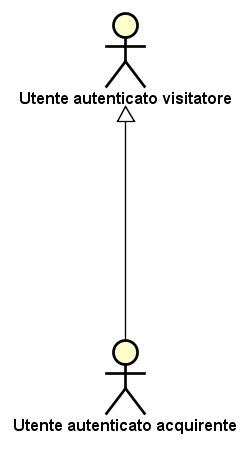
\includegraphics[scale=0.8]{utenti}
		\caption{Gerarchia degli utenti. L'utente autenticato acquirente può effettuare tutte le operazioni dell'utente registrato visitatore ma in più ha la possibilità di acquistare gli oggetti presenti nel carrello}
	\end{center}
\end{figure}
\FloatBarrier

\subsection{Casi d'uso}

Verranno di seguito elencati tutti i casi d'uso individuati dal \textit{team} che spiegano in che modo un utente possa interagire con l'applicazione. Per ogni caso d'uso viene mostrato uno schema \textit{UML}\ped{\hyperlink{uml}{G}} che ne rappresenta il flusso operativo. \\ 
Non vengono considerati i casi d'uso relativi alla registrazione al sito/e-commerce poiché tale funzionalità non è stata da me implementata non essendo di mia competenza.

\subsubsection{Caso d'uso UC1: Autenticazione}

\begin{itemize}
	\item \textbf{Attori:} utente registrato visitatore, utente registrato acquirente;
	\item \textbf{Descrizione:} prima di accedere all'ambiente virtuale, l'utente viene invitato ad immettere l'\textit{username} e la \textit{passowrd} scelti in fase di registrazione all'interno di una scena 2D. Potrà immettere tali dati manualmente utilizzando la normale tastiera del proprio telefono;
	\item \textbf{Precondizione:} l'applicazione è avviata e mostra la pagina di login;
	\item \textbf{Postcondizione:} l'autenticazione è andata a buon fine e l'applicazione passa in modalità \textit{VR}\ped{\hyperlink{vr}{G}}.
	\item \textbf{Scenario principale:}
	\begin{enumerate}
		\item L'utente può inserire l'\textit{username} (UC1.1);
		\item L'utente può inserire la \textit{passowrd} (UC1.2);
		\item L'utente può confermare i dati inseriti premendo sul pulsante di login (UC1.3).
	\end{enumerate}
	\item \textbf{Estensioni:} l'utente può visualizzare un messaggio di errore se i dati immessi non corrispondono a quelli di registrazione o se il campo \textit{username} e \textit{passowrd} sono vuoti (UC1.4).
\end{itemize}

\label{UC1}
\begin{figure}[ht]
	\begin{center}
		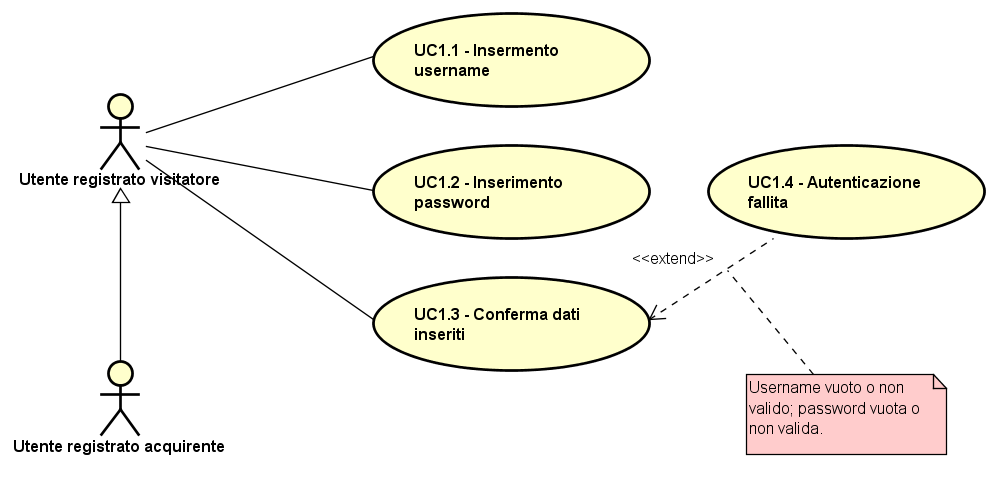
\includegraphics[scale=0.55]{usecase/uc1}
		\caption{UC1: Autenticazione}
	\end{center}
\end{figure}
\FloatBarrier

\subsubsection{Caso d'uso UC2: Interazione con l'ambiente virtuale}

\begin{itemize}
	\item \textbf{Attori:} utente registrato visitatore, utente registrato acquirente;
	\item \textbf{Descrizione:} l'utente, dopo l'autenticazione e collegato il telefono al visore, si ritrova ad osservare un ambiente virtuale. L'ambiente è formato da una stanza, la quale è visibile a 360 gradi se l'utente muove la testa mentre indossa il visore. Vi sono alcuni prodotti, segnalati da appositi marcatori, con i quali l'utente può interagire attivando un pannello informativo dove vengono visualizzati il nome, una descrizione, il prezzo e alcune foto. E' possibile aggiungere tali prodotti nel carrello, attivabile selezionando un'area segnalata da un'apposita scritta. I prodotti all'interno del carrello sonno acquistabili;
	\item \textbf{Precondizione:} l'utente ha effettuato con successo l'autenticazione;
	\item \textbf{Postcondizione:} l'utente interagisce con gli oggetti presenti nell'ambiente virtuale e se è acquirente può comprare gli oggetti presenti nel carrello;
	\item \textbf{Scenario principale:}
	\begin{enumerate}
		\item L'utente può interagire con un oggetto, segnalato da un apposito simbolo, presente nell'ambiente virtuale (UC2.1);
		\item L'utente può interagire con il carrello presente nell'ambiente e segnalato da un'apposita scritta (UC2.2);
		\item L'utente può uscire dall'applicazione effettuando così il logout (UC2.3).
	\end{enumerate}
\end{itemize}

\label{UC2}
\begin{figure}[ht]
	\begin{center}
		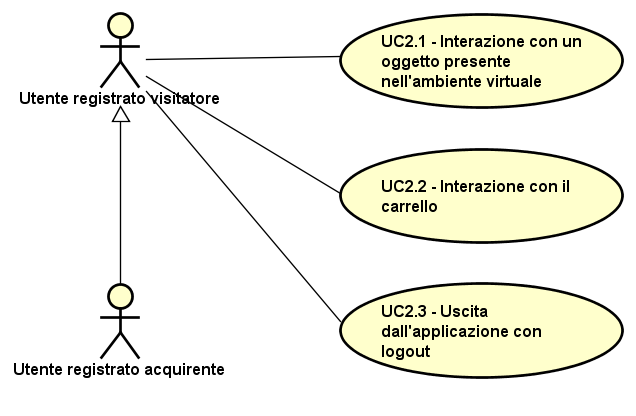
\includegraphics[scale=0.7]{usecase/uc2}
		\caption{UC2: Interazione con l'ambiente virtuale}
	\end{center}
\end{figure}
\FloatBarrier

\subsubsection{Caso d'uso UC2.1: Interazione con un oggetto}

\begin{itemize}
	\item \textbf{Attori:} utente registrato visitatore, utente registrato acquirente;
	\item \textbf{Descrizione:} l'utente interagisce con un oggetto presente nell'ambiente tramite l'interfaccia fisica del visore, attivando il pannello informativo. All'interno di questo sono riportate tutte le informazioni del prodotto e le sue foto. Dal pannello è possibile aggiungere l'oggetto al carrello;
	\item \textbf{Precondizione:} l'utente ha effettuato con successo l'autenticazione;
	\item \textbf{Postcondizione:} l'utente interagisce con l'oggetto attivando il pannello informativo.
	\item \textbf{Scenario principale:}
	\begin{enumerate}
		\item Visualizzazione informazioni dell'oggetto sul pannello informativo (UC2.1.1);
		\item Scorrimento foto dell'oggetto sul pannello informativo (UC2.1.2);
		\item Aggiunta oggetto al carrello selezionando l'apposito pulsante (UC2.1.3).
	\end{enumerate}
\end{itemize}

\label{UC2.1}
\begin{figure}[ht]
	\begin{center}
		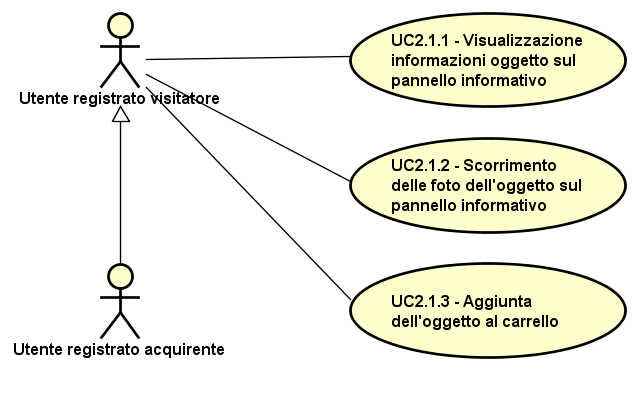
\includegraphics[scale=0.7]{usecase/uc2_1}
		\caption{UC2.1: Interazione con un oggetto}
	\end{center}
\end{figure}
\FloatBarrier

\subsubsection{Caso d'uso UC2.2: Interazione con il carrello}

\begin{itemize}
	\item \textbf{Attori:} utente registrato visitatore, utente registrato acquirente;
	\item \textbf{Descrizione:} entrambe le tipologie possono interagire con il carrello, segnalato nell'ambiente da un'apposita scritta. All'interno di esso sono visibili gli oggetti precedentemente inseriti. E' possibile, attraverso l'interfaccia fisica del visore, eliminarli uno ad uno o svuotare completamente il carrello. Se l'utente registrato è acquirente allora può procedere al pagamento;
	\item \textbf{Precondizione:} l'utente ha effettuato l'autenticazione;
	\item \textbf{Postcondizione:} l'utente visualizza i prodotti presenti nel carrello, potendoli acquistare se è acquirente;
	\item \textbf{Scenario principale:}
	\begin{enumerate}
		\item L'utente visualizza il pannello tridimensionale che rappresenta il carrello dove sono elencati i prodotti aggiunti precedentemente (UC2.2.1);
		\item L'utente può eliminare singolarmente un oggetto dal carrello (UC2.2.2);
		\item L'utente può svuotare completamente il carrello (UC2.2.3);
		\item Se l'utente è acquirente allora può procedere con l'acquisto dei prodotti (UC2.2.4).
	\end{enumerate}
\end{itemize}

\label{UC2.2}
\begin{figure}[ht]
	\begin{center}
		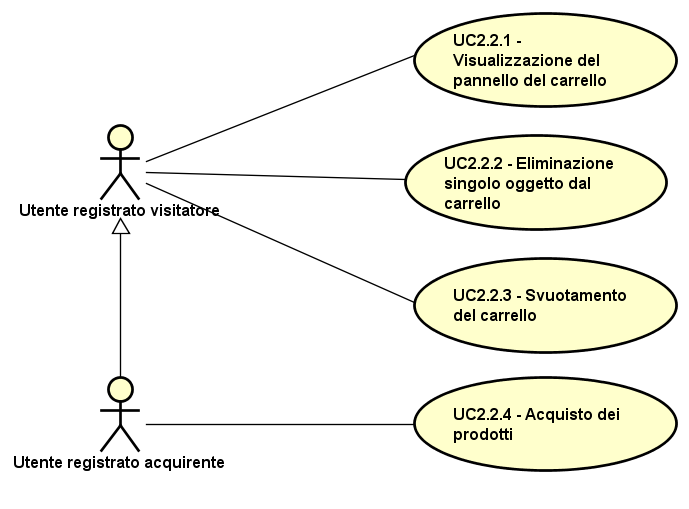
\includegraphics[scale=0.7]{usecase/uc2_2}
		\caption{UC2.2: Interazione con il carrello}
	\end{center}
\end{figure}
\FloatBarrier

\subsection{Requisiti}

Di seguito sono elencati tutti i requisiti funzionali che l'applicazione deve soddisfare in base ai casi d'uso trovati. Un requisito funzionale rappresenta una \textit{feature} che l'applicazione deve mettere a disposizione all'utente per garantirgli un'esperienza completa. \\
Ogni requisito funzionale è rappresentato da un codice identificativo RFx e da una descrizione che ne illustra lo scopo.

\begin{table}
	\centering
	\label{tabella-requisiti}
	\begin{tabular}{| l | p{10cm} |}
		\hline
		\textbf{Requisito} & \textbf{Descrizione} \\ \hline
		RF1 & L'applicazione deve permettere all'utente di potersi autenticare utilizzando \textit{username} e \textit{password} specificati in fase di registrazione. \\ \hline
		RF1.1 & L'applicazione deve permettere all'utente di inserire l'\textit{username}. \\ \hline
		RF1.2 & L'applicazione deve permettere all'utente di inserire la \textit{password}. \\ \hline
		RF1.3 & L'applicazione deve permettere all'utente di confermare i dati di autenticazione ed effettuare così il login. \\ \hline
		RF2 & L'applicazione deve permettere all'utente di visualizzare l'ambiente virtuale una volta indossato il visore e di interagire con esso. \\ \hline
		RF2.1 & L'applicazione deve permettere all'utente di interagire con un oggetto presente nella scena attraverso l'interfaccia fisica presente nel visore. \\ \hline
		RF2.1.1 & L'applicazione deve visualizzare le informazioni relative all'oggetto selezionato all'interno di un panello informativo posto davanti all'utente. \\ \hline
		RF2.1.2 & L'applicazione deve permettere la visualizzazione e lo scorrimento delle foto dell'oggetto selezionato all'interno del pannello informativo. \\ \hline
		RF2.1.3 & L'applicazione deve permettere l'aggiunta al carrello dell'oggetto selezionato. \\ \hline
		RF2.2 & L'applicazione deve permettere l'interazione col carrello segnalato da un'apposita scritta all'interno dell'ambiente virtuale. \\ \hline
		RF2.2.1 & L'applicazione deve visualizzare tutti gli oggetti presenti nel carrello precedentemente aggiunti. \\ \hline
		RF2.2.2 & L'applicazione deve permettere all'utente di eliminare un singolo oggetto dal carrello. \\ \hline
		RF2.2.3 & L'applicazione deve permettere di svuotare completamente il carrello. \\ \hline
		RF2.2.4 & L'applicazione deve permettere l'acquisto dei prodotti se l'utente è registrato acquirente. \\ 
		\hline
	\end{tabular}
	\caption{Tabella dei requisiti funzionali che l'applicazione deve soddisfare}
\end{table}
\FloatBarrier

\section{Progettazione}

Questa sezione descrive le più importanti e peculiari fasi di progettazione dell'applicazione. Molte delle decisioni prese sono state discusse da me assieme al \textit{team} di The White Dog s.r.l., cercando il più possibile di accontentare gli \textit{stakeholder}\hyperlink{sh}{\ped{G}}, ovvero il signor Stefano Mocellini, fondatore dell'azienda, attraverso l'ancora giovane e incompleta tecnologia \textit{VR}\ped{\hyperlink{vr}{G}}.

\subsection{Portabilità dell'applicazione}

Una delle sfide più impegnative di questo progetto era riuscire a sviluppare l'applicazione per entrambi i dispositivi: \textit{Samsung Gear VR} e \textit{Google Cardboard}. Prima di conoscere a basso livello tali tecnologie, avevamo progettato l'implementazione di un'interfaccia che riconoscesse la tecnologia in uso e che ne richiamasse così i metodi specifici. Purtroppo, dopo aver sperimentato gli \textit{SDK}\ped{\hyperlink{sdk}{G}} forniti da entrambe le piattaforme e seguito i due principali tutorial\footnote[1]{\textit{Samsung Gear VR:} \url{http://www.samsung.com/us/samsungdeveloperconnection/developer-resources/gear-vr.html} \\ \textit{Google Cardboard:} \url{https://developers.google.com/vr/unity/}}, mi sono reso conto che una totale portabilità non era possibile a causa delle forti differenze tra le due piattaforme. \\ \\
La prima differenza, e la più importante, è la \textbf{MainCamera} o Camera Principale. In un progetto \textit{Unity}, ogni scena possiede una o più camere che rappresentano il punto di vista dell'utente. Una camera normale non permette l'esperienza \textit{VR}\ped{\hyperlink{vr}{G}} poiché non è collegata ai sensori di movimento e rotazione del dispositivo. All'interno dei pacchetti \textit{Unity} offerti agli sviluppatori dalle due case, sono presenti le rispettive camere che, tramite script ad esse agganciati, permettono l'esperienza \textit{VR}\ped{\hyperlink{vr}{G}} una volta posizionate a piacimento all'interno della scena. Tali script si collegano direttamente ai sensori del dispositivo che è diverso per le due piattaforme. Il visore \textit{Samsung Gear VR} possiede al suo interno tutti i sensori di movimento e rotazione necessari e lo script, agganciato alla \textit{MainCamera}, legge i dati derivanti da essi. Invece, i dispositivi \textit{Google Cardboard} non possiedono alcun sensore e la \textit{MainCamera} legge i dati di rotazione e movimento direttamente dai sensori all'interno dello \textit{smartphone}. Questa profonda differenza hardware causa una forte differenza tra i due script della \textit{MainCamera}, obbligando ad inserire una camera specifica per ogni piattaforma all'interno della stessa scena.

\label{MainCamera}
\begin{figure}[ht]
	\begin{center}
		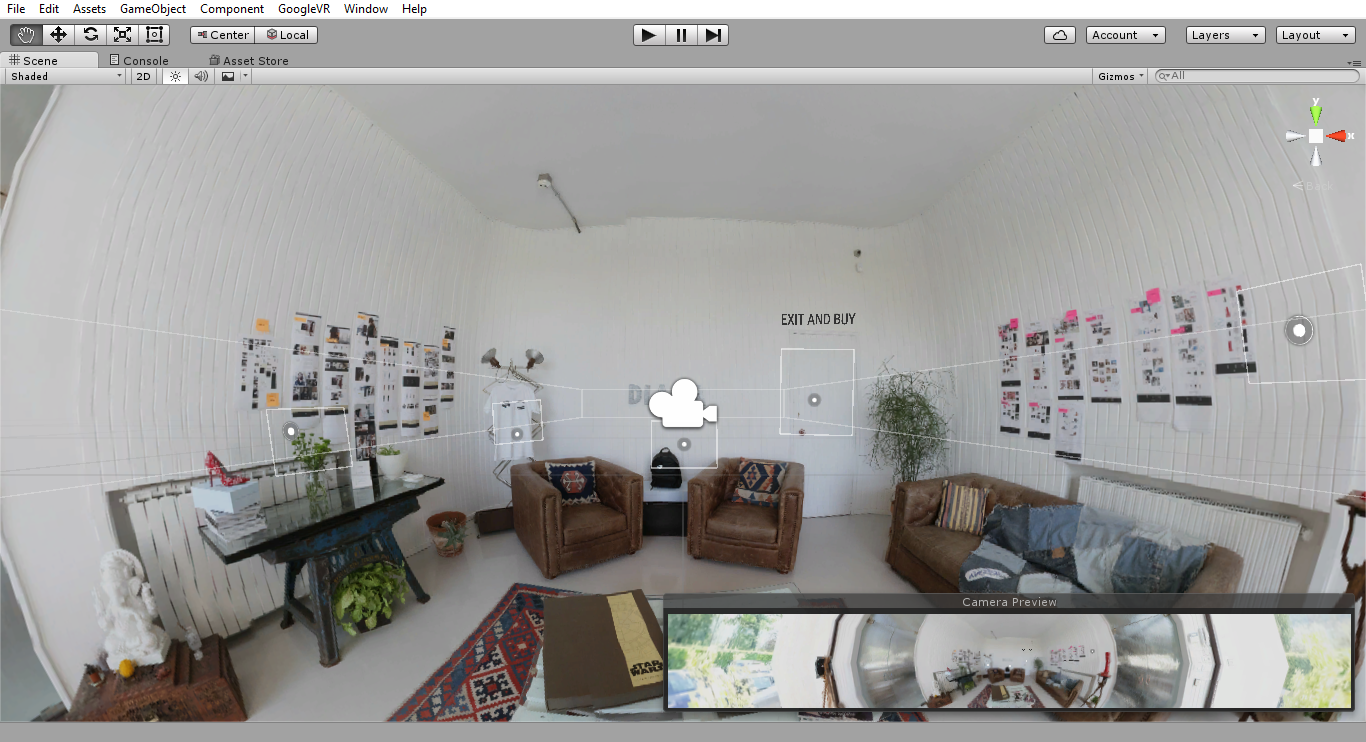
\includegraphics[scale=0.35]{maincamera}
		\caption{Camera VR posizionata all'interno dell'ambiente tridimensionale creato in Unity}
	\end{center}
\end{figure}
\FloatBarrier

La seconda importante differenza è l'implementazione degli \textbf{oggetti interattivi} all'interno della scena \textit{Unity}. Di base, sia per \textit{Samsung Gear VR} sia per \textit{Google Cardboard}, un oggetto per essere interattivo necessità di due caratteristiche:

\begin{itemize}
	\item \textbf{Mesh Collider:} è necessario aggiungere tale proprietà all'oggetto che si vuole rendere interattivo. Tale proprietà rende un oggetto "tangibile", ovvero può essere colliso da un altro oggetto presente nella scena. Questo permette alla \textit{Camera VR} di interagire con l'oggetto inviando un "raggio virtuale" verso quest'ultimo che, scontrandovisi, potrà attivare gli eventi che si desidera;
	\item \textbf{InteractiveScriptVR:} script, da agganciare all'oggetto, che cattura l'evento di selezione attraverso i metodi esposti dall'\textit{api} della particolare piattaforma. All'interno di questi metodi si può implementare il vero comportamento dell'oggetto interattivo.  
\end{itemize}

L'\texttt{InteractiveScriptVR} differisce profondamente da una piattaforma all'altra. \\
Per quanto riguarda \textit{Google Cardboard}, lo script implementa la classe \texttt{IGvrGazeResponder}, la quale espone i metodi per la cattura della selezione tramite lo spostamento del magnete posto lateralmente nel visore. \\
In \textit{Samsung Gear VR} invece, l'\texttt{InteractiveScriptVR} non implementa alcuna interfaccia ma necessita l'utilizzo del namespace \texttt{VRStandardAsset.Utils} per richiamare i metodi esposti dallo script \texttt{VRInteractiveItem}, script che va agganciato all'oggetto assieme all'\texttt{InteractiveScriptVR}. \\
Questa differenza di implementazione degli oggetti interattivi rende davvero difficoltosa la loro portabilità da una piattaforma all'altra. Dunque, dopo una lunga discussione avvenuta nell'ufficio R\&D, abbiamo deciso di abbandonare la totale portabilità dell'applicazione, raggiungendo però un compromesso: la separazione della cattura dell'evento di selezione dall'effettivo comportamento dell'oggetto, implementandoli in due script differenti. Il primo, che cambia da piattaforma a piattaforma, richiama il secondo dopo aver catturato l'evento di selezione, il quale rappresenta il vero comportamento dell'oggetto ed è indipendente dalla piattaforma in uso. In questo modo è stato possibile creare dei \textit{prefabs} (oggetti portabili all'interno dell'ambiente \textit{Unity} contenenti le informazioni di forma, colore, script agganciati eccetera) che contenessero solo le informazioni del comportamento dell'oggetto dopo la cattura della selezione.    

\subsection{Usabilità dell'applicazione}

La fase di acquisto inizialmente prevista comprendeva l'immissione dei propri dati di pagamento all'interno dell'ambiente \textit{VR}\ped{\hyperlink{vr}{G}} tramite una tastiera tridimensionale posta davanti all'utente, dove ogni tasto era selezionabile attraverso l'interfaccia fisica del visore. Dopo la sperimentazione di tale tastiera, abbiamo constatato la sua scarsa usabilità, causando un processo d'acquisto lungo e tedioso. Abbiamo dunque optato per una soluzione più semplice: l'utente prima di entrare nella scena \textit{VR}\ped{\hyperlink{vr}{G}} viene invitato a immettere i propri dati di login attraverso la normale tastiera del telefono, così da accedere al proprio account personale. Tale account deve essere precedentemente creato nel sito/e-commerce dedicato, dove possono essere immessi anche i dati di pagamento. L'implementazione di tale sito esce dagli obiettivi di questo progetto, dunque non mi sono occupato dello sviluppo di quest'ultimo. Una volta autenticato, lo \textit{smartphone} passa in modalità \textit{VR}\ped{\hyperlink{vr}{G}}, invitando l'utente ad indossare il visore. All'interno dell'ambiente, all'utente non viene più richiesto di immettere dati, così da poter sperimentare in tutta serenità l'esperienza virtuale. \\
Questa soluzione però ha mostrato al \textit{team} la profonda differenza tra le piattaforme \textit{Samsung Gear VR} e \textit{Google Cardboard}. Ogni applicazione \textit{Samsung Gear VR}, una volta avviata, richiede all'utente di inserire lo \textit{smartphone} all'interno del visore prima di poter effettivamente essere utilizzata. Questo obbliga lo sviluppatore a prevedere tutte scene di tipo \textit{VR}\ped{\hyperlink{vr}{G}} durante lo sviluppo dell'applicazione, contrariamente a \textit{Google Cardboard} che permette la coesistenza di tutte le tipologie scenografiche: 2D, 3D e \textit{VR}\ped{\hyperlink{vr}{G}}. Dunque, non è stato possibile inserire una scena 2D iniziale di login per la piattaforma Samsung e, a causa dei tempi ridotti di stage, non ho potuto sviluppare una soluzione a tale problema.

\label{Login}
\begin{figure}[ht]
	\begin{center}
		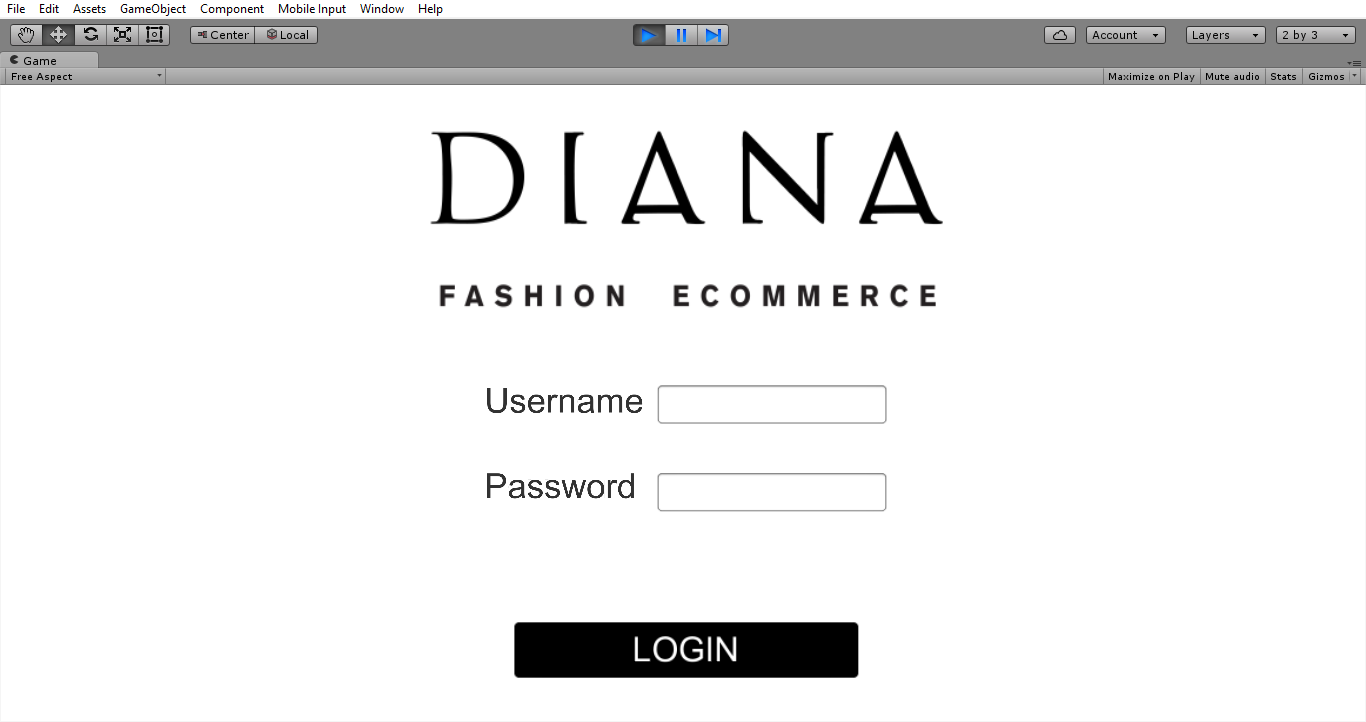
\includegraphics[scale=0.35]{login}
		\caption{Schermata 2D di login}
	\end{center}
\end{figure}
\FloatBarrier

\subsection{Costruzione della scena 3D}

Dopo un'attenta fase di ricerca iniziale sulla tecnologia \textit{Unity} e \textit{VR}\ped{\hyperlink{vr}{G}}, ho potuto constatare che vi sono due modi principali per costruire una scena 3D:

\begin{itemize}
	\item \textbf{Tramite modellazione 3D dell'intero ambiente virtuale};
	\item \textbf{Tramite l'applicazione di una foto a 360 gradi di una stanza ad una sfera o cubo inversi}.
\end{itemize}

La prima soluzione permette una vera esperienza 3D, dando la possibilità all'utente di spostarsi nelle tre dimensioni, prevedendo l'utilizzo di un gamepad. Ogni oggetto è ben definito in un punto dello spazio tridimensionale e osservabile da tutte le angolazioni. Purtroppo però per costruire un ambiente 3D di qualità accettabile sono necessarie profonde conoscenze di modellazione, conoscenze che fuoriescono dall'obiettivo di questo stage. \\
La seconda soluzione non permette una totale esperienza 3D, poiché applica una foto 2D a 360 gradi ad una sfera o un cubo inversi creati in \textit{Unity}. L'effetto così creato simula la tridimensionalità, non permettendo all'utente lo spostamento tra gli oggetti ma solo una visione stereoscopica della stanza. Il livello qualitativo raggiunto però è ottimo, se la foto viene realizzata con le giuste apparecchiature. Abbiamo deciso dunque di utilizzare la seconda metodologia per la creazione dell'ambiente. \\
Abbiamo così realizzato la foto a 360 gradi utilizzando una macchinetta fotografica di alta qualità presente nell'azienda seguendo la guida presente nel sito lightspacewater\footnote[2]{\url{http://www.lightspacewater.net/Tutorials/PhotoPano2/paper/}}. \\
Posizionata la macchinetta fotografica sul cavalletto al centro di una stanza, appositamente arredata allo scopo nell'azienda Diana Corp., abbiamo effettuato 3 foto, una sovraesposta, una sottoesposta e una ad esposizione normale, ogni 45 gradi orizzontalmente. Abbiamo poi ripetuto l'operazione inclinando la macchinetta 45 gradi verso il basso ed infine 45 gradi verso l'alto. \\ 
Le foto così ottenute, ci hanno permesso di creare la foto a 360 gradi tramite il software Autopano\footnote[3]{\url{http://www.kolor.com/autopano/}}, che l'ha creata automaticamente a meno di qualche punto di agganciamento inserito manualmente. Infine abbiamo applicato la foto come texture di una sfera inversa creata tramite l'editor di \textit{Unity}.

\label{Sfera}
\begin{figure}[ht]
	\begin{center}
		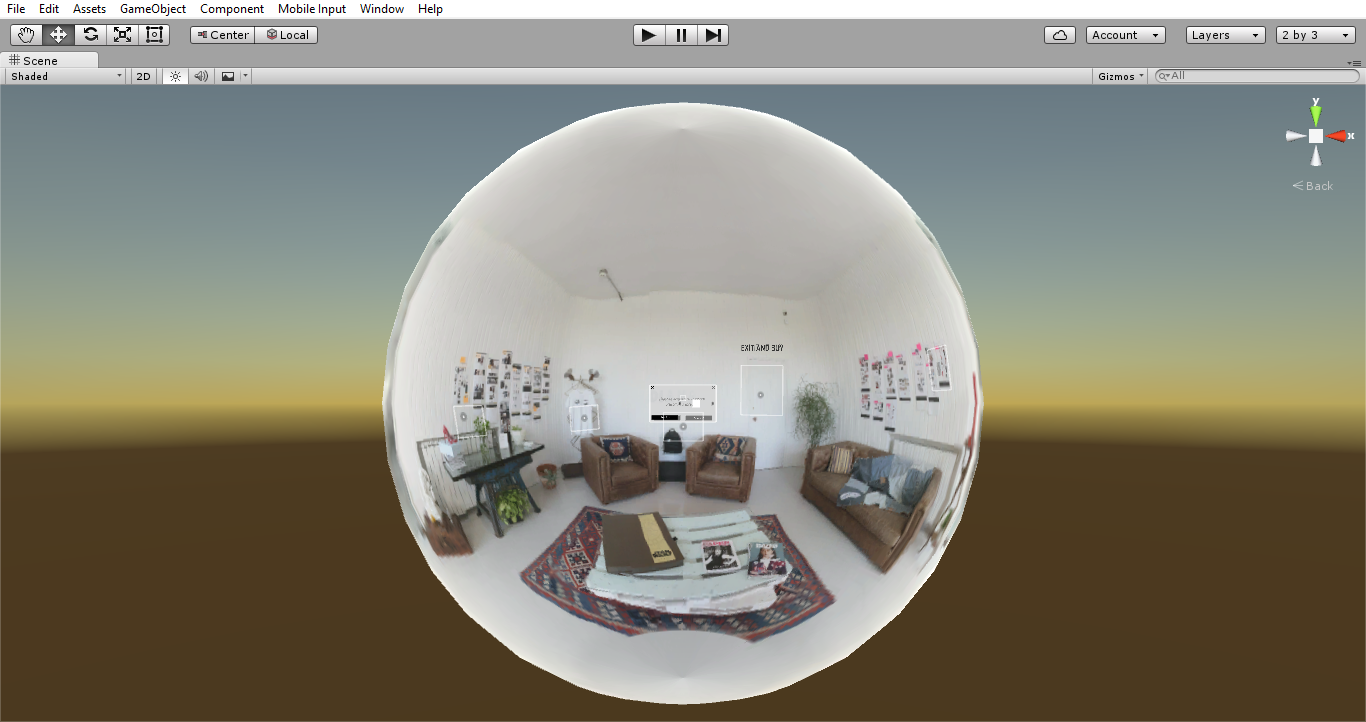
\includegraphics[scale=0.35]{sfera}
		\caption{Sfera inversa a cui è stata applicata la foto 360 della stanza come texture}
	\end{center}
\end{figure}
\FloatBarrier  

\subsection{Interazione con gli oggetti all'interno della scena} 

All'interno della scena creata tramite la foto a 360 gradi, gli oggetti presenti nella stanza non sono veri oggetti tridimensionali modellati in \textit{Unity}. A quest'ultimi, come descritto nella sezione 3.5.1, è possibile applicare la proprietà \textit{Mesh Collider}, per renderli tangibili, e lo script che cattura l'evento di selezione. Purtroppo nella soluzione da noi adottata gli oggetti fanno parte della foto che crea lo sfondo, perciò non è possibile applicargli queste due proprietà. \\
Abbiamo così deciso di porre davanti ad ogni oggetto un pannello tridimensionale creato tramite l'editor di \textit{Unity} e ad esso agganciargli le caratteristiche citate. In più al pannello viene disabilitata la proprietà \textit{Mesh Renderer}, proprietà che lo rende visibile. \\ 
In questo modo viene simulata l'interattività dell'oggetto che, alla selezione tramite l'interfaccia fisica del visore, attiva il pannello informativo relativo all'oggetto selezionato.

\label{Oggetto Interattivo}
\begin{figure}[ht]
	\begin{center}
		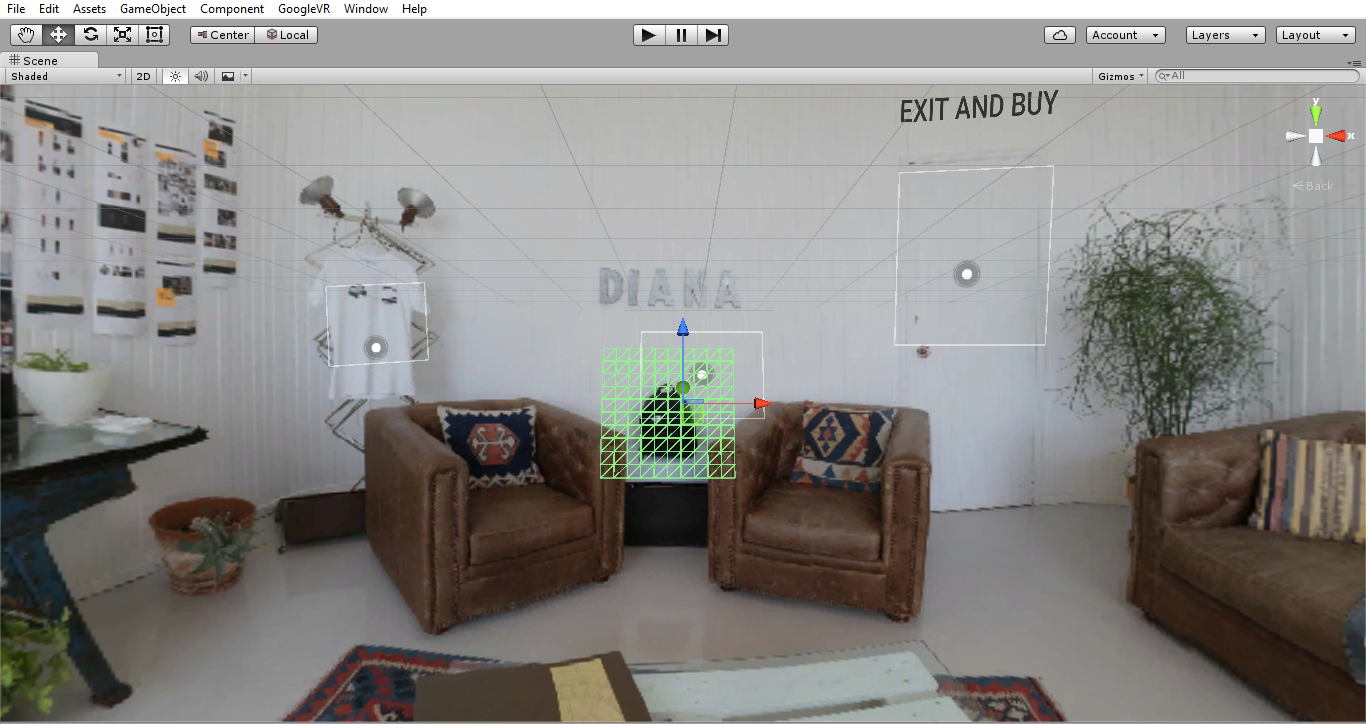
\includegraphics[scale=0.35]{pannello}
		\caption{Pannello tridimensionale posto davanti ad un oggetto presente nella stanza per renderlo interattivo}
	\end{center}
\end{figure}
\FloatBarrier  

\subsection{Progettazione e integrazione con AWS API Gateway}

Uno degli obiettivi dello stage era sperimentare la comunicazione tra l'applicazione creata con \textit{Unity} e sistemi esterni tramite protocollo HTTP, come ad esempio un \textit{e-commerce}. Per testare tali funzionalità in sicurezza, senza dover creare o modificare gli \textit{e-commerce} aziendali, il tutor mi ha suggerito di utilizzare il servizio \textit{API Gateway} di \textit{Amazon Web Service}. \\ 
Amazon API Gateway è un servizio completamente gestito che semplifica agli sviluppatori la creazione, la pubblicazione, la manutenzione, il monitoraggio e la protezione delle API su qualsiasi scala. Essa agisce come porta d'entrata attraverso la quale le applicazioni possono accedere a dati, logica di business o funzionalità dei servizi di back-end. Gestisce tutte le attività di accettazione ed elaborazione relative alle chiamate API simultanee, inclusi gestione del traffico, controllo di accessi e autorizzazioni, monitoraggio e gestione delle versioni delle API. Infine permette la creazione di \textit{API Mock}, ovvero API che non si agganciano ad alcun back-end ma che rispondono messaggi prefissati ad ogni chiamata HTTP. Quest'ultima funzionalità ci ha spinto ad utilizzare questo servizio, dato che lo sviluppo di un vero back-end non rientrava all'interno degli obiettivi di stage. \\
Ho creato dunque tre risorse e al loro interno le relative chiamate HTTP:
\begin{itemize}
	\item \textbf{/login}: risorsa riguardante le operazioni di autenticazione. Contiene la chiamata:
	\begin{itemize}
		\item POST: riceve un file JSON contenente l'username e la password immesse dall'utente e restituisce un \textit{token} di autenticazione.
	\end{itemize}
	\item \textbf{/products}: risorsa riguardante le operazione sui prodotti. Contiene la chiamata:
	\begin{itemize}
		\item GET: ritorna un file JSON contenente le informazioni riguardanti tutti i prodotti all'interno della scena come nome, descrizione e foto.
	\end{itemize}
	\item \textbf{/products/{id}}: risorsa riguardante le operazioni su un singolo prodotto. Contiene la chiamata:
	\begin{itemize}
		\item GET: ritorna un file JSON contenente le informazioni su un singolo prodotto in base all'id passato. 
	\end{itemize}
	\item \textbf{/cart}: risorsa riguardante le operazioni sul carrello. Contiene le chiamate:
	\begin{itemize}
		\item POST: riceve un file JSON contenente i prodotti presenti all'interno del carrello.
	\end{itemize} 
\end{itemize}

\label{AWS API Gateway}
\begin{figure}[ht]
	\begin{center}
		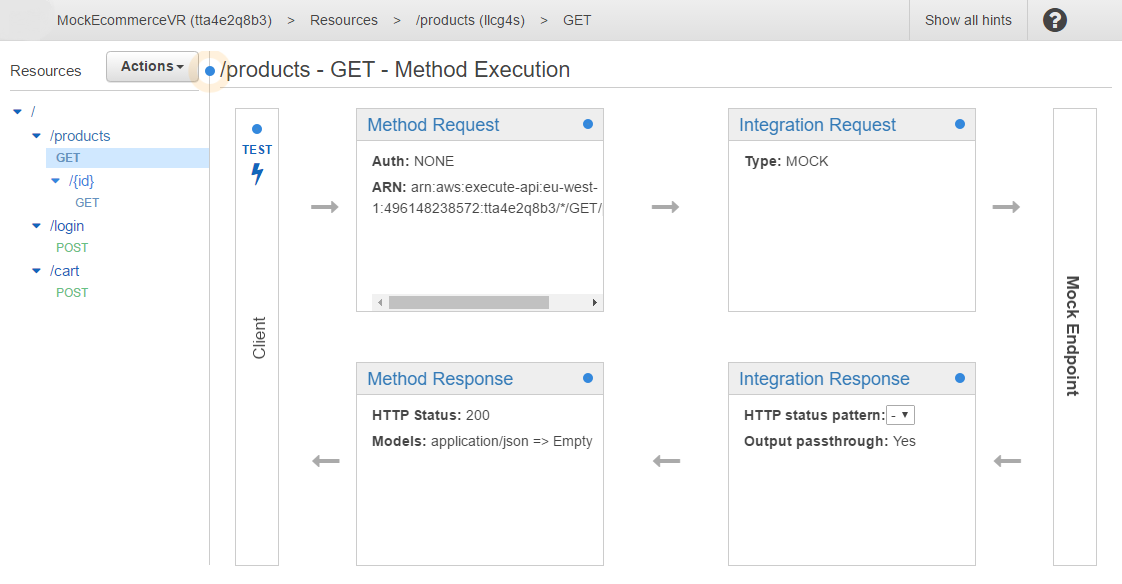
\includegraphics[scale=0.45]{aws}
		\caption{Flusso della chiamata GET all'interno della risorsa \textit{/products} in AWS API Gateway}
	\end{center}
\end{figure}
\FloatBarrier

Per quanto riguarda \textit{Unity}, invece, ho sfruttato la classe \texttt{WWW} che consente di effettuare chiamate GET per recuperare dati JSON o foto:

\begin{lstlisting}[style=MyCStyle]
// Endpoint GET creato tramite API Gateway che restituisce un file
// JSON contenente le informazioni sui prodotti
string url = "https://execute-api.amazonaws.com/prod/products";

// Costruzione dell'oggetto WWW e passaggio dell'endpoint come
// singolo parametro
WWW www = new WWW(url);
yield return www;

// Recupero delle informazioni 
string info = www.text;
\end{lstlisting}
 
e chiamate POST, potendo inviare \textit{headers} e corpo:

\begin{lstlisting}[style=MyCStyle]
// Endpoint POST creato tramite API Gateway che riceve i dati
// di login e restituisce un token di autenticazione
string url = "https://execute-api.amazonaws.com/prod/login";

// Creazione del file JSON
string JSON = "{\"username\" : " + "\"" + Username + "\", "
	+ "\"password\" : " + "\"" + Password + "\"}";	
byte[] body = System.Text.Encoding.UTF8.GetBytes(JSON);

// Creazione degli headers necessari per il riconoscimento
// del file JSON
Dictionary<string, string> headers = 
	new Dictionary<string, string>();
headers.Add("Content-Type", "application/json");	
headers.Add("X-HTTP-Method-Override", "POST");

// Costruzione dell'oggetto WWW e passaggio dell'endpoint come
// singolo parametro
WWW www = new WWW(url, body, headers);
yield return www;
\end{lstlisting}

\section{Sviluppo}

Questa sezione descrive nel dettaglio il personale sviluppo delle più importanti funzionalità dell'applicazione attraverso l'editor grafico e il linguaggio di scripting C\# offeri dal \textit{framework}\ped{\hyperlink{fw}{G}} \textit{Unity}.


\subsection{Dati persistenti attraverso le scene}

L'applicazione sviluppata possiede due scene: la prima offre una schermata di login dove l'utente può digitare la propria \textit{username} e \textit{password}; la seconda permette la visualizzazione dell'ambiente virtuale dopo aver indossato il visore. \textit{Unity} prevede la possibilità di creare più scene all'interno dello stesso progetto e il passaggio tra queste è gestibile attraverso script che caricano la scena successiva dopo aver catturato un particolare evento. Nel mio specifico caso, dopo che l'utente ha digitato l'\textit{username} e la \textit{password} e selezionato il pulsante di login, viene effettuata la chiamata POST all'API contenete le due informazioni digitate. Se la chiamata va a buon fine, viene restituito un \textit{token} di autenticazione e viene così caricata la scena \textit{VR}\ped{\hyperlink{vr}{G}}. \\
Il \textit{token} di autenticazione serve all'utente in fase di acquisto dei prodotti, il quale permette al sistema di riconoscere quest'ultimo associandogli i dati di pagamento immessi in fase di registrazione. Purtroppo però, di default, \textit{Unity} distrugge ogni oggetto presente all'interno di una scena prima di passare a quella successiva. Questo comportamento non è accettabile per il \textit{token} di autenticazione, il quale deve vivere fino alla fase di acquisto. Ho creato dunque un oggetto generico, o \textit{Empty Object}, all'interno della prima scena di autenticazione e attraverso il metodo \texttt{DontDestroyOnLoad ()}, offerto da \textit{Unity}, l'ho reso persistente:

\begin{lstlisting}[style=MyCStyle]
public class UserSessionScript : MonoBehaviour {

	private string token;

	// Il metodo Awake() deriva dalla classe MonoBehaviour
	// e al suo interno e' possibile impostare
	// tutte le caratteristiche iniziali che l'oggetto
	// deve avere prima che la scena abbia inizio
	void Awake () {
	DontDestroyOnLoad (this);
	}
	
	public string getToken() {
		return token;
	}
	
	public void setToken(string token) {
		this.token = token
	}
}
\end{lstlisting}

In questo modo, l'oggetto \textit{UserSession} sarà presente nella scena successiva e si potrà così recuperare le informazioni che contiene. Questa operazione, però, necessita di un'altro script di \textit{utilities} per recuperare l'oggetto a runtime all'interno di una scena nella quale prima non era presente:

\begin{lstlisting}[style=MyCStyle]
public class UserSessionUtils : MonoBehaviour {

	// Il metodo Find() offerto da Unity permette 
	// di recuperare il riferimento di un oggetto
	// all'interno della scena passandogli il nome
	// come parametro
	public string getUserToken() {
	GameObject userSession = GameObject.Find("UserSession");
	return userSession.GetComponent<UserSessionScript>().getToken();
	}

	public void setUserToken(string token) {
	GameObject userSession = GameObject.Find("UserSession");
	userSession.GetComponent<UserSessionScript>().setToken(token);
	}
}
\end{lstlisting}

Dunque, una volta recuperato il \textit{token} di autenticazione dalla chiamata POST, è possibile memorizzarlo all'interno dell'oggetto \textit{UserSession} tramite lo script \textit{UserSessionUtilities} e caricare così la scena successiva:

\begin{lstlisting}[style=MyCStyle]
	WWW www = new WWW(url, body, headers);
	yield return www;
	
	// JsonData e' una classe che effettua il  
	// parsing degli oggetti JSON in Unity. In questo  
	// caso recupera il token di autenticazione
	JsonData jsonvale = JsonMapper.ToObject(www.text);
	string username = jsonvale ["token"].ToString ();
	
	UserSessionUtils usu = new UserSessionUtils ();
	usu.setUserToken (token);
	
	// Metodo che carica la scena denominata 1
	// in fase di compilazione
	SceneManager.LoadScene (1);
\end{lstlisting}

\subsection{Il pannello informativo}
\textit{Unity} permette la creazione di due principali tipologie di oggetti all'interno di una scena:

\begin{itemize}
	\item \textbf{3D Object:} oggetti sviluppati nelle tre dimensioni che possono contenere le informazioni di forma, colore, tangibilità, rigidità, comportamento eccetera. \\
	Un esempio di questi oggetti è rappresentato dal cubo, dalla sfera o dal cilindro. Questi elementi possono essere modificati e assemblati per creare ambienti e oggetti sempre più complessi;
	\item \textbf{UI:} oggetti 2D che compongono l'interfaccia utente, ovvero pannelli dove è possibile scrivere e scorrere un testo, visualizzare un'immagine, selezionare pulsanti eccetera.
\end{itemize}

Per la creazione del pannello informativo ho fatto ampio utilizzo di questa seconda tipologia di oggetti, trovandola adatta allo scopo. \\
Per costruire un'interfaccia utente in \textit{Unity} è necessario innanzitutto la presenza dell'oggetto \textit{EventSystem} all'interno della scena. Tale oggetto permette la gestione degli eventi, catturando i vari input provenienti da qualsiasi terminale come mouse, tastiera, gamepad o, in questo caso, dispositivo \textit{VR}\ped{\hyperlink{vr}{G}}. Sia Samsung che Google offrono una loro versione di tale oggetto, dato che i possibili input di \textit{Samsung Gear VR} sono più numerosi rispetto a quelli di \textit{Google Cardboard}. \\
Per poter essere visibili e interattivi, ogni oggetto UI deve essere figlio di un oggetto \textit{Canvas}. Il \textit{Canvas}, di default, è visibile come un pannello opaco all'interno della scena e serve sostanzialmente a raggruppare gli oggetti UI per farli comunicare con l'\textit{EventSystem}. \\
Vi sono tre tipologie di \textit{Canvas}:

\begin{itemize}
	\item \textbf{Screen Space - Overlay:} questa modalità di \textit{rendering} pone gli elementi dell'interfaccia utente fissi all'interno della scena e davanti alla camera dell'utente. Se lo schermo viene ridimensionato o viene cambiata la risoluzione, il \textit{Canavs} cambierà automaticamente dimensioni per adattarsi;
	\item \textbf{Screen Space - Camera:} questà modalità di \textit{rendering} è molto simile alla \textit{Screen Space - Overlay}, con l'unica differenza che è possibile scegliere la distanza e l'inclinazione degli oggetti UI rispetto alla camera;
	\item \textbf{World Space:} questa modalità di \textit{rendering} è profondamente differente dalle prime due poiché premette di visualizzare gli oggetti UI in un qualsiasi punto dello spazio tridimensionale, potendoli riposizionare a runtime.
\end{itemize}

Data la varietà di punti interattivi all'interno della stanza tridimensionale, ho ritenuto necessario l'utilizzo della modalità \textit{World Space}, poiché desideravo che il pannello si potesse posizionare davanti ad ogni oggetto interattivo alla selezione di quest'ultimo.

\label{Pannello informativo}
\begin{figure}[ht]
	\begin{center}
		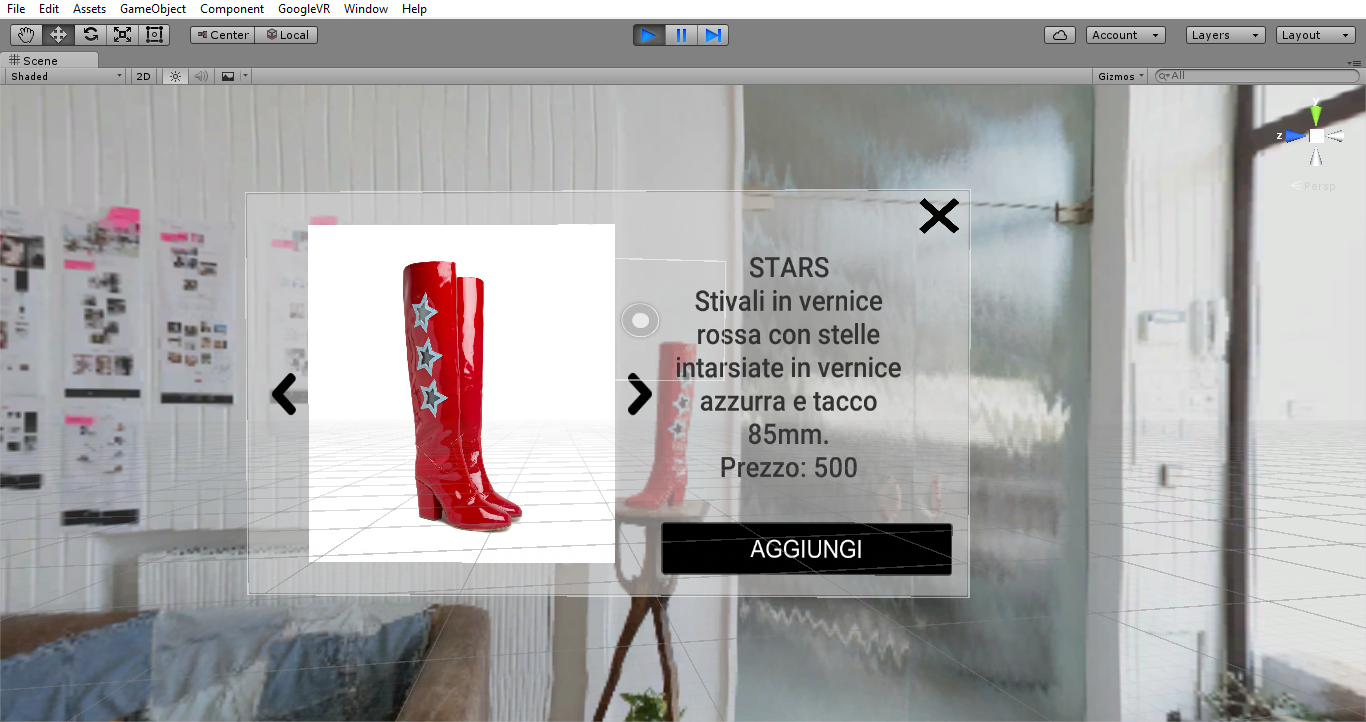
\includegraphics[scale=0.35]{pannello-stivali}
		\caption{Pannello informativo attivato dopo la selezione di un particolare oggetto all'interno della scena}
	\end{center}
\end{figure}
\FloatBarrier

Per quanto riguarda il suo spostamento nello spazio tridimensionale, inizialmente avevo previsto come punto di partenza il centro della sfera, disattivando ovviamente la proprietà \textit{Mesh Renderer} che ne permette la visualizzazione. Alla selezione di un oggetto presente nella stanza, lo script che gestisce il pannello calcola il punto medio tra l'oggetto e l'osservatore e vi si posiziona, mostrando le informazioni. Purtroppo però, gli oggetti UI non possiedono tale proprietà e se si desidera renderli invisibili è necessario disattivarli del tutto tramite il metodo \texttt{SetActive()}. Questo pone un nuovo problema: non è possibile riferirsi ad un oggetto disattivato per riattivarlo a runtime. \\
La soluzione finale trovata e discussa col \textit{team} di sviluppatori, non è sicuramente ottimale ma è funzionale. Tale problema rischiava di non farmi rispettare il piano di lavoro concordato e c'erano ancora molti punti che necessitavano di essere esplorati e sperimentati. Abbiamo quindi deciso che il punto d'origine e di ritorno del pannello sarebbe stato esterno alla sfera. In questo modo esso sarebbe rimasto sempre attivo fin dall'inizio ma invisibile poiché esterno alla stanza tridimensionale.

\label{Pannello sfera}
\begin{figure}[ht]
	\begin{center}
		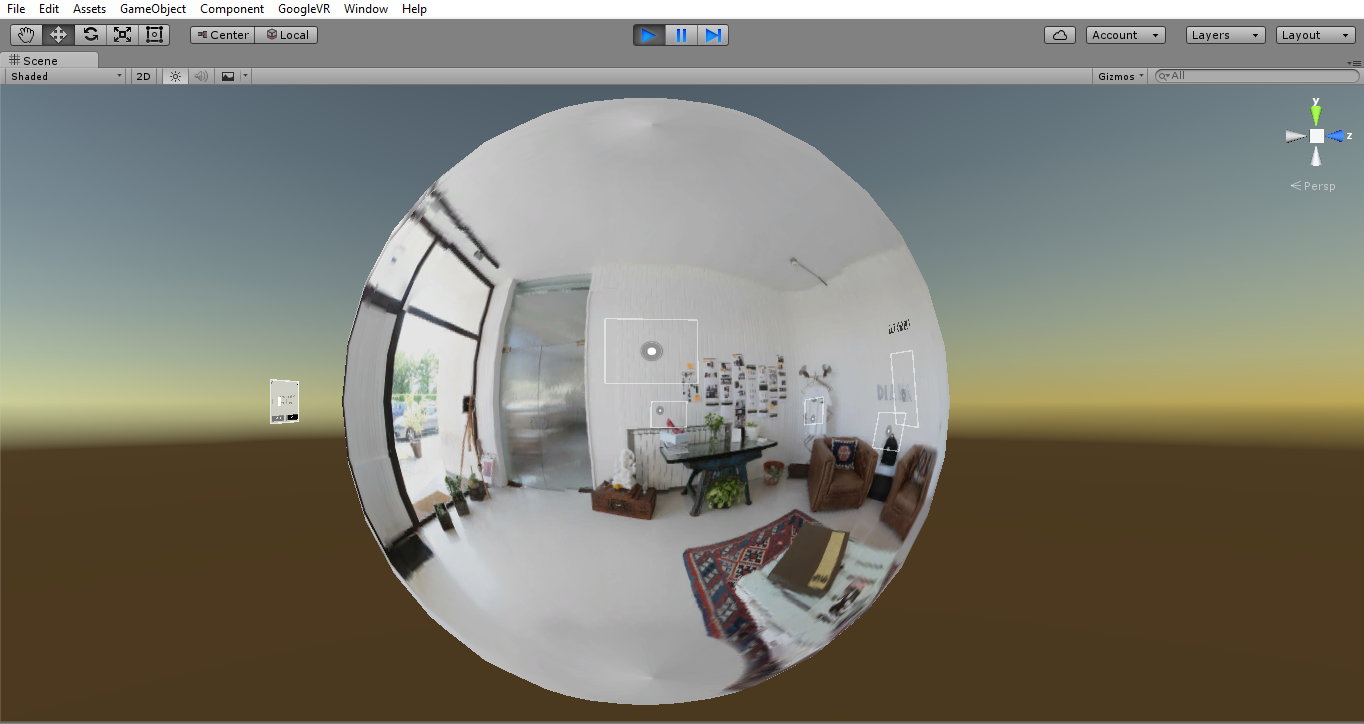
\includegraphics[scale=0.35]{pannello-sfera}
		\caption{Pannello informativo attivo all'esterno della sfera}
	\end{center}
\end{figure}
\FloatBarrier 

\subsection{Creazione e parsing di oggetti JSON in Unity}

\textit{Unity} offre al programmatore la classe \texttt{JsonUtility} che permette la trasformazione di un oggetto in una stringa JSON:

\begin{lstlisting}[style=MyCStyle]
MyClass myObject = new MyClass();
myObject.level = 1;
myObject.timeElapsed = 47.5f;
myObject.playerName = "Dr Charles Francis";

string json = JsonUtility.ToJson(myObject);
// la stringa json e' uguale a: 
// {"level":1,"timeElapsed":47.5,"playerName":"Dr Charles Francis"}
\end{lstlisting}

e viceversa:

\begin{lstlisting}[style=MyCStyle]
string json = {"level":1,"timeElapsed":47.5,
	"playerName":"Dr Charles Francis"};
MyClass myObject = JsonUtility.FromJson<MyClass>(json);
\end{lstlisting}

Purtroppo però, non viene offerta alcuna funzionalità di parsing di file JSON, a me necessaria per leggere le informazioni dei prodotti recuperate tramite la chiamata GET all'API. Dopo alcune ricerche, ho scoperto l'esistenza della libreria LitJSON\footnote[4]{\url{https://lbv.github.io/litjson/}}, libreria scritta in C\# e compatibile con tutti i linguaggi .Net. Essa, dopo aver importato il file \textit{LitJSON.dll} all'interno del progetto Unity, permette di leggere il file JSON scaricato come se fosse un semplice array, accedendo direttamente ai vari campi tramite le doppie parentesi quadre:

\begin{lstlisting}[style=MyCStyle]
// Chiamata GET per il recupero delle infomrazioni di un prodotto
www = new WWW (url);
yield return www;

// Crea un parser per il file JSON scaricato
jsonvale = JsonMapper.ToObject(www.text);

id = jsonvale ["id"].ToString ();

name = jsonvale ["name"].ToString ();

description = jsonvale ["description"].ToString ();

price = jsonvale ["price"].ToString ();

text = name + "\n" + description + "\n" + "Prezzo: " + price;

// Il file JSON contiene i link per sacricare le immagini
www_img1 = new WWW (jsonvale ["img1"].ToString ());
yield return www_img1;
imageArray [0] = www_img1.texture;

www_img2 = new WWW (jsonvale ["img2"].ToString ());
yield return www_img2;
imageArray [1] = www_img2.texture;

www_img3 = new WWW (jsonvale ["img3"].ToString ());
yield return www_img3;
imageArray [2] = www_img3.texture;
\end{lstlisting}

\subsection{Creazione a runtime di oggetti interattivi}

Per la realizzazione del carrello interattivo è stato necessario uno studio approfondito sulla creazione di oggetti scenici a runtime in \textit{Unity}. Questo perché inizialmente il carrello deve risultare vuoto e riempirsi a mano a mano che l'utente decide di aggiungere un prodotto, ovvero mentre la scena è in \textit{play mode}. \\ 
La soluzione adottata prevede la creazione, tramite l'editor grafico, di un pannello UI generico contenente i componenti per la foto, per il nome e per il prezzo dell'ipotetico prodotto che sarà aggiunto al carrello. All'oggetto grafico così creato, viene agganciato lo script \texttt{ListItemController} contenente i campi logici del pannello che verranno riempiti con le informazioni dello specifico prodotto: 

\begin{lstlisting}[style=MyCStyle]
public class ListItemController : MonoBehaviour {
	private string id;

	private Text description;

	private Image icon;

	public string getId() {
		return id;
	}

	public void setId(string id) {
		this.id = id;
	}
	
	public Text getDescription() {
		return description;
	}
	
	public void setDescription(Text description){
		this.description = description;
	}
	
	public Image getIcon() {
		return icon;
	}
		
	public void setIcon(Image icon){
		this.icon = icon;
	}
}
\end{lstlisting}

Il pannello grafico e lo script agganciato vengono uniti in un unico pacchetto per formare un \textit{prefab} di nome \textit{ListItem}, ovvero un oggetto prefabbricato pronto per essere istanziato all'interno della scena. Così, lo script incaricato alla gestione del carrello grafico, ovvero \texttt{ListController}, dopo aver controllato tutti i prodotti presenti nel carrello logico, gestito dallo script \texttt{ShoppingBagScript}, instanzia tanti \textit{ListItem} quanti sono i prodotti presenti nel carrello logico e li posizione in lista all'interno del pannello del carrello:

\begin{lstlisting}[style=MyCStyle]
public void printItem(Item[] items) {
	// Per ogni oggetto presente nel pannello logico
	// che non e' stato ancora stampato nel carrello
	while (alreadyItemPrint < 
		shoppingBag.GetComponent<ShoppingBagScript> ().getCounter ()) {

	// Istanzia l'oggetto prefab all'interno della scena
	GameObject newItem = 
		Instantiate (ListItemPrefab) as GameObject;
	ListItemController controller = 
		newItem.GetComponent<ListItemController> ();

	// Recupera le informazioni del prodotto logico per 
	// inizializzare il pannello grafico del prodotto
	controller.setId(items [alreadyItemPrint].getId ());
	controller.setDescrtiption(items [alreadyItemPrint].getInfo ());
	controller.setIcon(Sprite.Create (items [alreadyItemPrint].getImg (), 
		new Rect (0, 0, items [alreadyItemPrint].getImg ().width, 
		items [alreadyItemPrint].getImg ().height), new Vector2 (0.5f, 0.5f));

	// Posiziona ogni prodotto in lista all'interno
	// del pannello del carrello
	newItem.transform.SetParent (ContentPanel.transform);
	newItem.transform.position += new Vector3 (0, 0, 32);
	newItem.transform.rotation = ContentPanel.transform.rotation;
	newItem.transform.localScale = Vector3.one;

	// Se l'array dei prodotti e' pieno
	// effettua il resize
	if (alreadyItemPrint == ItemPrefabs.Length) {
		GameObject[] newItemPrefabs = 
			new GameObject [ItemPrefabs.Length * 2];
		for (int i = 0; i < ItemPrefabs.Length; i++) {
			newItemPrefabs [i] = ItemPrefabs [i];
		}
		ItemPrefabs = newItemPrefabs;
	}
	ItemPrefabs [alreadyItemPrint] = newItem;
	alreadyItemPrint++;
	}
}
\end{lstlisting}

\label{Carrello}
\begin{figure}[ht]
	\begin{center}
		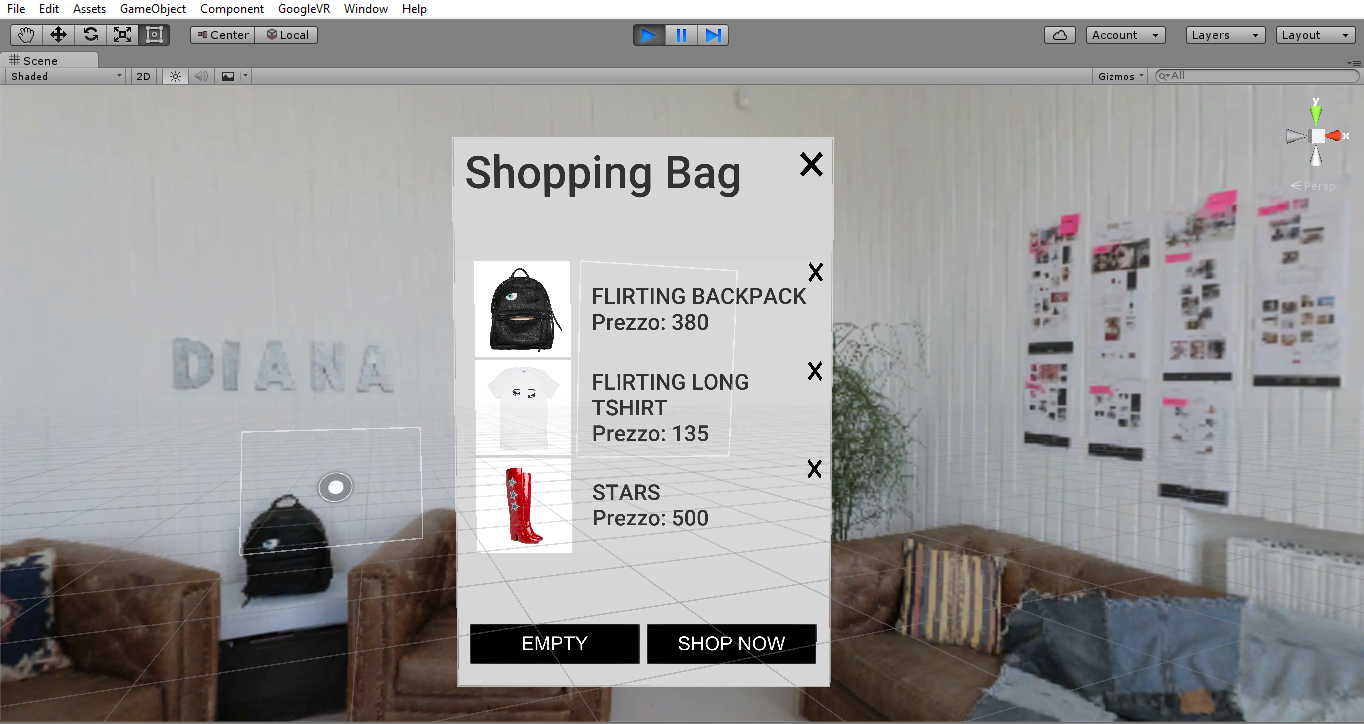
\includegraphics[scale=0.35]{carrello}
		\caption{Carrello riempito dei prodotti presenti nella stanza}
	\end{center}
\end{figure}
\FloatBarrier 

\section{Verifica e validazione}

La natura di questo progetto di stage è di pura sperimentazione. Fin dalla prima riunione, assieme al tutor aziendale, mi è stato esplicitamente confermato che l'azienda non pretendeva un prodotto finito, dato che nemmeno il \textit{team} di ricerca e sviluppo sapeva se fosse realizzabile, ma solo uno studio sulle tecnologie \textit{VR}\ped{\hyperlink{vr}{G}} disponibili e se queste potessero essere utilizzate nel mondo \textit{e-commerce}. Molto tempo perciò è stato dedicato alla sperimentazione delle tecnologie \textit{VR}\ped{\hyperlink{vr}{G}} presenti in azienda, sia nell'utilizzo dell'harware che del software, per decidere quale tra queste fosse la più adatta per lo scopo. Oltretutto, la mia conoscenza iniziale sulla computer grafica era praticamente nullo e ho trascorso molto tempo a studiare il \textit{framework}\ped{\hyperlink{fw}{G}} \textit{Unity} per riuscire a costruire manualmente, tramite l'editor, tutti gli oggetti grafici presenti nella scena. Questo mi ha portato a sviluppare non un'applicazione completa, da poter un giorno completare e rilasciare nei maggiori \textit{store}, ma un insieme di funzionalità che testano fino a dove la tecnologia per la realtà virtuale è integrabile con il mondo \textit{e-commerce}. Per questi motivi le attività di verifica e validazione non sono state pianificate nel piano di lavoro e, a causa sia dell'obbiettivo di stage che dei tempi ristretti, non sono state nemmeno effettuate. 